\chapter*{Software Design}
This section provides architectural details regarding the software design supporting DERP.

\section*{Overview}
\begin{center}
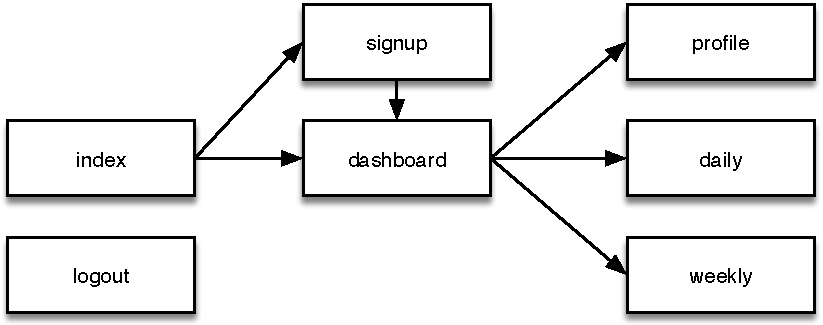
\includegraphics[width=0.8\textwidth]{./pageflow.pdf}
\end{center}

The page flow for DERP is presented in the figure above. The logout page can be accessed by the user selecting to logout or when an error is detected in the user's session. Page names match the names of the implementing functions in \emph{app.py}.

\section*{Pages}
\subsection*{index}
This page is the entry point to DERP and redirects the user based on some checks. If a user must be authenticated, \emph{index} will handle the authentication via GitHub Oauth. 
When handling authentication, \emph{index} will set the initial values for the user's DERP session.

The user should go from \emph{index} to \emph{signup}, \emph{dashboard}, xor \emph{logout}.

\subsubsection*{Entry Conditions}
Access to this page is unrestricted.

\subsubsection*{Exit Conditions}
\begin{description}
\item[signup] The user session has a reasonable GitHub credential in the session but no registered Duck Id.
\item[dashboard] The user session has a reasonable GitHub credential and matching registered Duck Id.
\item[logout] There is a miss match between GitHub credential and Duck Id in the user session.
\end{description}


\subsection*{logout}
This page is used to clear the DERP user session. GitHub Oauth uses the GitHub cookie, which DERP cannot touch. Logging out does not change the GitHub user associated with the user's browser.

\subsubsection*{Entry Conditions}
Access to this page is unrestricted.

\subsubsection*{Exit Conditions}
The user session will be cleared.


\subsection*{signup}
This page adds a user to the DERP database. The GitHub username is acquired from the session and the Duck Id cannot be changed after submission. Signup also requires a repository URL and preferred email address.

\subsubsection*{Entry Conditions}
\begin{enumerate}
\item Valid github\_username in the user session.
\item github\_username is not present in the database.
\end{enumerate}

\subsubsection*{Exit Conditions}
\begin{enumerate}
\item github\_username and duck\_id are set in the user session.
\item User record has been stored in the database.
\end{enumerate}


\subsection*{dashboard}
This page is the user's homepage in the system.

\subsubsection*{Entry Conditions}
\begin{enumerate}
\item Valid github\_username in the user session.
\item Valid duck\_id in the user session.
\item github\_username and duck\_id match a user record.
\end{enumerate}

\subsubsection*{Exit Conditions}
None

\subsection*{profile}
This page allows user settings to be viewed and changed.

\subsubsection*{Entry Conditions}
\begin{enumerate}
\item Valid github\_username in the user session.
\item Valid duck\_id in the user session.
\item github\_username and duck\_id match a user record.
\end{enumerate}

\subsubsection*{Exit Conditions}
Submitted updates are stored in the database.


\subsection*{daily}
This page allows user's to view and add daily status reports.

\subsubsection*{Entry Conditions}
\begin{enumerate}
\item Valid github\_username in the user session.
\item Valid duck\_id in the user session.
\item github\_username and duck\_id match a user record.
\end{enumerate}

\subsubsection*{Exit Conditions}
Submitted updates are stored in the database.


\subsection*{weekly}
This page allows user's to view and add weekly status reports.

\subsubsection*{Entry Conditions}
\begin{enumerate}
\item Valid github\_username in the user session.
\item Valid duck\_id in the user session.
\item github\_username and duck\_id match a user record.
\end{enumerate}

\subsubsection*{Exit Conditions}
Submitted updates are stored in the database.


\section*{Supporting Code}
Functionality in this section is organized by the file it appears in.

\subsection*{derp.wsgi}
\emph{derp.wsgi} wraps \emph{app.py} so that mod\_wsgi can start DERP correctly. 

\subsection*{picklesession.py}
Apache wsgi may run several Flask instances concurrently, which is a problem for the default Flask session implementation. \emph{picklesession.py} implements a server side session that is visible across Flask instances on the same host by extending the Flask SessionInterface.

\subsection*{app.py}
All of the Flask routes are defined in \emph{app.py}. Additionally, \emph{app.py} contains some helper functions.

\subsubsection{is\_login\_ok(userclass=`any')}
This function performs the check used by most pages to verify that the user session contains correct information and is authorized to view the page. The following checks must pass for \emph{is\_login\_ok} to return True.
\begin{enumerate}
\item A github\_username is in the session.
\item A duck\_id is in the session.
\item The github\_username and duck\_id occur together in the database.
\item The user is of class \emph{userclass}
\end{enumerate}